\section{Variable Time Step (VTS)}  
%==============================================================================
Variable time step simulations are possible using standard MATLAB ODE solvers.
A semi-complete and partially-detailed explanation of the functions and code used to make this happen will \emph{probably} be written in a separate document `later'\ldots

Explain FTS and VTS

Cover speed up possibility

explain zeroing derivatives.

\textbf{NOTE:} Variable time step simulation is still experimental and should be used with caution.


%------------------------------ from vts explained
%==============================================================================
\subsection{Solver Control Array (solver\_con)}  
Theoretically, a user will only have to add a \verb|solver_con| to a valid data file to use variable time step methods.
If a \verb|solver_con| is not specified, Huen's method is used for all time blocks (i.e. default PST behavior).

Between each \verb|sw_con| entry, a \emph{time block} is created that is then solved using a the defined solution method in the \verb|solver_con|.
As such, the \verb|solver_con| array has 1 less row than the \verb|sw_con| array.
An example \verb|solver_con| array (with code comments) is shown below.
\begin{minted}[
		frame=lines,
		framesep=2mm,
		baselinestretch=1.2,
		bgcolor=gray!13,
		fontsize=\footnotesize,
		%linenos,
		breaklines
		]{MATLAB}
%% solver_con format
% A cell with a solver method in each row corresponding to the specified
% 'time blocks' defined in sw_con
%
% Valid solver names:
% huens - Fixed time step default to PST
% ode113 - works well during transients, consistent # of slns, time step stays relatively small
% ode15s - large number of slns during init, time step increases to reasonable size
% ode23 - realtively consistent # of required slns, timstep doesn't get very large
% ode23s - many iterations per step - not efficient...
% ode23t - occasionally hundereds of iterations, sometimes not... decent
% ode23tb - similar to 23t, sometimes more large solution counts

solver_con ={ ...
    'huens'; % pre fault - fault
    'huens'; % fault - post fault 1
    'huens'; % post fault 1 - post fault 2
    'huens'; % post fault 2 - sw_con row 5
    'huens'; % sw_con row 5 - sw_con row 6 
    'ode23t'; % sw_con row 6  - sw_con row 7  (end)
    };
\end{minted}

As of this writing, the pstSETO version uses the \verb|s_simu_BatchVTS| script to perform variable time stepping methods.
This script will likely replace the \verb|s_simu| script in the main PST4 folder after versioning is complete.\\

%==============================================================================
\subsection{MATLAB ODE Solvers}
The variable time step implementation in PST revolves around using the built in MATLAB ODE solvers.
All these methods perform actions depicted in the following block diagram.

\begin{figure}[!h]
	\centering
	\footnotesize
	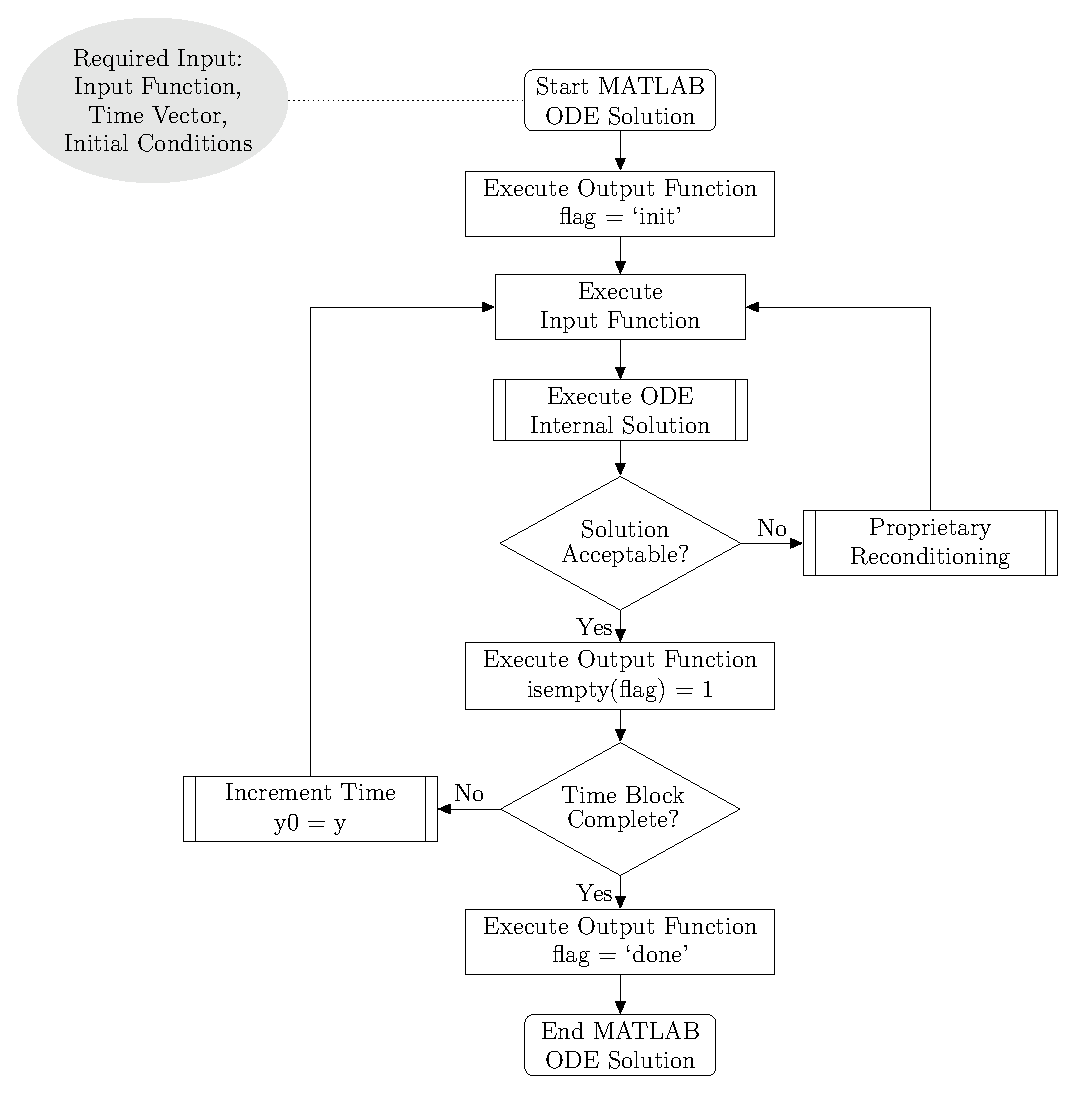
\includegraphics[width=.8\linewidth]{./../../one-offs/200804-ODEblockDiagram/200804-ODEblockDiagram}
	\caption{MATLAB ODE block diagram.}
	\label{fig: MATLAB ode block diagram}
\end{figure}%\vspace{-1 em}

The input to an ODE solver include, an input function, a time interval (time block), initial conditions, and solver options.
The current options used for VTS are shown below and deal with error tolerance levels, initial step size, max step size, and an Output function.

\begin{minted}[
		frame=lines,
		framesep=2mm,
		baselinestretch=1.2,
		bgcolor=gray!13,
		fontsize=\footnotesize,
	%	linenos,
		breaklines
				]{MATLAB}
% Configure ODE settings
%options = odeset('RelTol',1e-3,'AbsTol',1e-6); % MATLAB default settings
options = odeset('RelTol',1e-4,'AbsTol',1e-7, ...
    'InitialStep', 1/60/4, ...
    'MaxStep',60, ...
    'OutputFcn',outputFcn); % set 'OutputFcn' to function handle
\end{minted}

%==============================================================================
\subsubsection{vtsInputFcn} 
The slightly abbreviated (mostly complete) input function is shown below.
\begin{minted}[
		frame=lines,
		framesep=2mm,
		baselinestretch=1.2,
		bgcolor=gray!13,
		fontsize=\footnotesize,
	%	linenos,
		breaklines
				]{MATLAB}
function [dxVec] = vtsInputFcn(t, y)
% VTSINPUTFCN passed to ODE solver to perfrom required step operations
%
%   NOTES: Updates and returns g.vts.dxVec
%
%   Input:
%   t - simulation time
%   y - solution vector (initial conditions)
%
%   Output:
%   dxVec - requried derivative vector for ODE solver
global g

%% call handleStDx with flag==2 to update global states with newest passed in soln.
% write slnVec vector of values to associated states at index k
% i.e. update states at g.vts.dataN with newest solution
handleStDx(g.vts.dataN, y, 2)

%% Start initStep action ==================================================
initStep(g.vts.dataN)

%% Start of Network Solution ==============================================
networkSolutionVTS(g.vts.dataN, t)

%% Start Dynamic Solution =================================================
dynamicSolution(g.vts.dataN )

%% Start of DC solution ===================================================
dcSolution(g.vts.dataN )

%% save first network solution
if g.vts.iter == 0
    handleNetworkSln(g.vts.dataN ,1)
end

g.vts.iter = g.vts.iter + 1; % increment solution iteration number

handleStDx(g.vts.dataN , [], 1) % update g.vts.dxVec
dxVec = g.vts.dxVec; % return updated derivative vector
end % end vtsInputFcn
\end{minted}

%==============================================================================

\subsubsection{vtsOutputFcn} 
The slightly abbreviated output function is shown below.
\begin{minted}[
		frame=lines,
		framesep=2mm,
		baselinestretch=1.2,
		bgcolor=gray!13,
		fontsize=\footnotesize,
	%	linenos,
		breaklines
				]{MATLAB}
function status = vtsOutputFcn(t,y,flag)
% VTSOUTPUTFCN performs associated flag actions with ODE solvers.
%
%   Input:
%   t - simulation time
%   y - solution vector
%   flag - dictate function action
%
%   Output:
%   status - required for normal operation (return 1 to stop)

global g 
status = 0; % required for normal operation

if isempty(flag) % normal step completion
    % restore network to initial solution
    handleNetworkSln(g.vts.dataN ,2) % may cause issues with DC.
    
    monitorSolution(g.vts.dataN); % Perform Line Monitoring and Area Calculations 
    
    %% Live plot call
    if g.sys.livePlotFlag
        livePlot(g.vts.dataN)
    end
    
    % after each successful integration step by ODE solver:
    g.vts.dataN = g.vts.dataN+1;    % increment logged data index 'dataN'
    g.sys.t(g.vts.dataN) = t;       % log step time
    g.vts.stVec = y;                % update state vector
    handleStDx(g.vts.dataN, y, 2)   % place new solution results into associated globals
    
    g.vts.tot_iter = g.vts.tot_iter + g.vts.iter;   % update total iterations
    g.vts.slns(g.vts.dataN) = g.vts.iter;           % log solution step iterations
    g.vts.iter = 0;                                 % reset iteration counter
    
elseif flag(1) == 'i' 
    % init solver for new time block
    g.sys.t(g.vts.dataN) = t(1);    % log step time
    handleStDx(g.vts.dataN, y, 2)   % set initial conditions
  
elseif flag(1) == 'd'
    % only debug screen output at the moment
end % end if
end % end function
\end{minted}

%==============================================================================
\subsection{Functions for Variable Time Step Integration}  
A number of new functions were created to allow for VTS to be integrated into PST.
Some functions were simply portions of code previously located in \verb|s_simu| and placed into a function for ease of use and clarity of code flow, while others were created to handle data or perform other tasks specifically related to VTS.
The following sub paragraphs provide some information about such functions that have not been previously introduced.
% related VTS functions

%==============================================================================
\subsubsection{handleNetworkSln}  
The \verb|handleNetworkSln| function was created to store, and restore, calculated values set to globals during a network solution.
The purpose of this function was to allow for the first network solution performed each step to be carried forward after multiple other network solutions may over-write the calculated values at the same data index.
This over-writing may occur during the MATLAB ODE solvers repeated call to the input function.
As shown below, \verb|handlNetworkSln| takes a data index \verb|k| and an operation \verb|flag| as inputs.
\begin{minted}[
		frame=lines,
		framesep=2mm,
		baselinestretch=1.2,
		bgcolor=gray!13,
		fontsize=\footnotesize,
	%	linenos,
		breaklines
				]{MATLAB}
function handleNetworkSln(k, flag)
% HANDLENETWORKSLN saves or restores the network solution at data index k
%
%   NOTES: Used to reset the newtork values to the initial solution in VTS.
%
%   Input:
%   k - data index to log from and restore to
%   flag - choose funtion operation
%       0 - initialize globals used to store data
%       1 - collect newtork solution values from index k into a global vector
%       2 - write stored network solution vector to network globals data at index k
\end{minted}

%==============================================================================
\subsubsection{handleStDx}  
The \verb|handleStDx| function was created to perform the required state and derivative handling to enable the use internal MATLAB ODE solvers.
Its general operation is probably best described via the internal function documentation provided below.

\begin{minted}[
		frame=lines,
		framesep=2mm,
		baselinestretch=1.2,
		bgcolor=gray!13,
		fontsize=\footnotesize,
	%	linenos,
		breaklines
				]{MATLAB}
function handleStDx(k, slnVec, flag)
% HANDLESTDX Performs required state and derivative handling for ODE solvers
%
%   NOTES:  Requires state and derivative values are in the same g.(x) field.
%           Not all flags require same input.
%
%   Input:
%   k - data index
%   flag - choose between operations
%           0 - initialize state and derivative cell array, count states
%           1 - update g.vts.dxVec with col k of derivative fields
%           2 - write slnVec vector of values to associated states at index k
%           3 - update g.vts.stVec with col k of state fields
%   snlVec - Input used to populate states with new values
\end{minted}

The new global structure created in the SETO version of PST enables this function to complete the stated operations by relying heavily on dynamic field names. 
Essentially, all required field names, sub-field names, and states are collected into a cell (flag operation 0) that is then iterated through to collect data from, or write data to the appropriate location (all other flag operations).

The usefulness of \verb|handleStDx| is that the standard MATLAB ODE solvers require a single derivative vector as a returned value from some passed in `input function', and each PST model calculates derivatives and places them into various globals. 
Thus, a derivative collection algorithm was needed (flag operation 1).
Once the ODE solver finishes a step, the returned solution vector (of integrated states) must then be parsed into the global state variables associated with the supplied derivatives (flag operation 2).
At the beginning of time blocks that use the MATLAB ODE solvers, an initial conditions vector of all the states related to the derivative vector is required (flag operation 3).

To avoid handling function output, global vectors \verb|g.vts.dxVec| and \verb|g.vts.stVec| are used to hold updated derivative and state vector information.

It should be noted that original PST globals follow the same data structure,
however, new models (such as AGC and pwrmod/ivmmmod) use a slightly different data structure and must be handled in a slightly different way.
As of this writing AGC and pwrmod functionality has been added to \verb|handleStDx| and it seems very possible to add more models that require integration as they arise.





%==========================================================
%\subparagraph{vtsInputFcn and vtsOutputFcn}  
%These functions were described earlier.


\begin{comment}
Document Section 'templates'
%==========================================================
\subparagraph{FcnName}  
FcnDescription
\begin{minted}[
		frame=lines,
		framesep=2mm,
		baselinestretch=1.2,
		bgcolor=gray!13,
		fontsize=\footnotesize,
	%	linenos,
		breaklines
				]{MATLAB}
PasteNewCodeHere
\end{minted}

%==========================================================
\begin{minted}[
		frame=lines,
		framesep=2mm,
		baselinestretch=1.2,
		bgcolor=gray!13,
		fontsize=\footnotesize,
	%	linenos,
		breaklines
				]{MATLAB}
PasteNewCodeHere
\end{minted}
%==========================================================

\end{comment}